
  
\section{Experiments and Results}
\label{ex_and_re}
In this section, we present a comprehensive, E2E evaluation of the LLM inference performance on our IMAX accelerator. 
We compare the measured performance of our FPGA prototype and the projected performance of a potential \SI{28}{\nano\meter} ASIC implementation against a state-of-the-art high-performance GPU, a general-purpose GPU with a comparable process node, and a dedicated edge AI GPU. 
The primary objective of these experiments is to quantitatively evaluate the performance and energy efficiency of the IMAX architecture. 
This analysis focuses on the fundamental trade-off between performance and power consumption.


\subsection{Experimental Setup}
\begin{figure}[t]
  \centering
  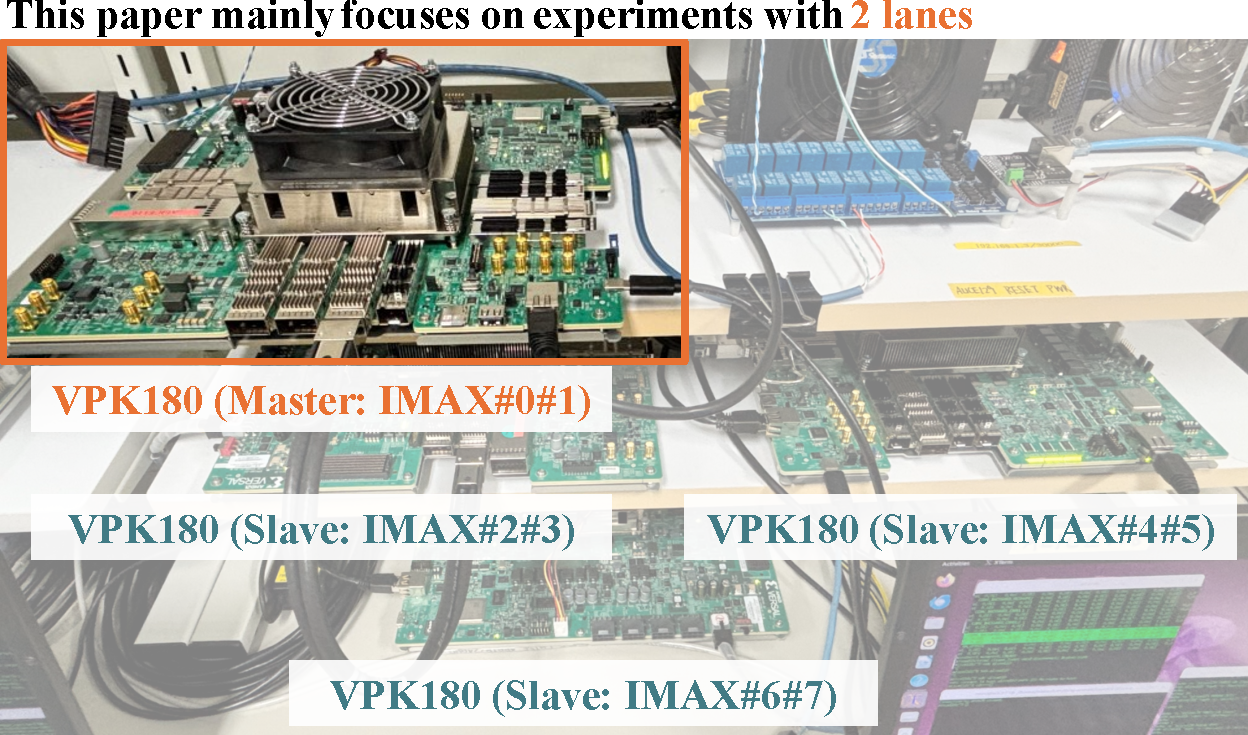
\includegraphics[width=1\columnwidth]{./imax3_proto.pdf}
  \caption{The experimental setup for the IMAX3 FPGA prototype, featuring a multi-board configuration with four AMD Versal VPK180 evaluation kits.}
  \label{fig:imax3_proto}
  % \vspace{-2em}
\end{figure}

  
We compare the performance of our IMAX accelerator against several commercial platforms. 
As shown in Fig.~\ref{fig:imax3_proto}, we implemented the IMAX prototype on an AMD Versal Premium VPK180 evaluation kit using Vivado 2024.1. 
This prototype consists of an eight-lane IMAX operating at \SI{145}{\mega\hertz} and uses an Arm Cortex-A72 PS as the host.
Although the FPGA supports up to eight IMAX lanes, our main evaluation uses a two-lane configuration. 
A preliminary analysis revealed that the dual-core ARM host becomes a performance bottleneck beyond two lanes, limiting the accelerator's utilization. 
This two-lane setup was therefore chosen to isolate the accelerator's performance from the host system. 
The architecture's scalability and the impact of host performance are further analyzed in Section~\ref{discussion}.
To evaluate the future potential of the architecture, we projected its performance as a \SI{28}{\nano\meter} ASIC. 
This projection is based on the established methodology from our previous work\nobreak\cite{imax3}, where we performed a detailed static timing and power analysis using Synopsys Design Compiler\cite{SynopsysNDDCUltra}. 
The analysis utilized the TSMC \SI{28}{\nano\meter} process technology, including its standard cell libraries and wireload models, and assumed \SI{10}{\percent} average switching activity for power estimation. 
From this analysis, we determined that a maximum operating frequency of \SI{840}{\mega\hertz} is achievable, which represents an approximately \num{6}$\times$ speedup over the FPGA implementation.
For the \SI{64}{K\byte} LMM configuration adopted in our evaluation, the power was calculated to be \SI{2.16}{\watt} for the FP16 kernel, \SI{4.41}{\watt} for Q8\_0, \SI{4.88}{\watt} for Q3\_K, and \SI{6.1}{\watt} for Q6\_K. 
Our commercial comparison platforms include a modern high-performance GPU system (NVIDIA RTX 4090), a previous-generation GPU system (NVIDIA GTX 1080 Ti), and an edge AI device (NVIDIA Jetson AGX Orin). 
The GTX 1080 Ti was selected to provide a comparison against a widely adopted GPU manufactured on a \SI{16}{\nano\meter} process, which is closer to our \SI{28}{\nano\meter} ASIC projection. 
Detailed hardware specifications are summarized in Table~\ref{tab:processor_comparison_annotated}.
The software and operating system configurations for each platform were standardized to ensure a fair comparison:
\begin{itemize}
\item The IMAX FPGA prototype runs a PetaLinux distribution, cross-compiled for the 64-bit ARM (aarch64) architecture.
\item Both the NVIDIA RTX 4090 and GTX 1080 Ti systems operate on Ubuntu 22.04.5 LTS with CUDA Toolkit 12.4.
\item The NVIDIA Jetson AGX Orin uses the JetPack R36.4.4 software stack.
\end{itemize}
All platforms were benchmarked using an identical version of the llama.cpp framework and the exact same quantized model files. 
This rigorous setup eliminates variations from the software stack and model data, allowing for a direct comparison of the underlying hardware architectures. 


To establish a consistent baseline for comparing energy efficiency, our power model utilizes nominal specifications.
For the IMAX (\SI{28}{\nano\meter}) ASIC projection, the total power during offloaded phases is calculated based on synthesis results. 
Specifically, the active power is determined by multiplying the power estimated from synthesis by the number of active lanes (two in our primary evaluation). 
The total system power is then calculated by adding the measured idle power of the host CPU to this active power value. 
This model distinguishes between host-primary processing and phases where the IMAX cores are active.
For the commercial GPU/CPU platforms, we model active power using their official Thermal Design Power (TDP) values applying either the host CPU's base or peak TDP\cite{Intel_Xeon_w5-2455X_Specs} depending on which component is primarily active. 
This approach enables us to assess the potential energy efficiency of each architecture operating within its specified maximum power budget.
While TDP does not represent average power consumption, it provides a standardized metric for comparing performance under peak load conditions. 
The NVIDIA Jetson AGX Orin was evaluated in its nominal \SI{60}{\watt} maximum performance mode. 
We acknowledge this methodological choice as a limitation and discuss its implications in Section~\ref{discussion}.

We executed a diverse set of LLM inference workloads on these platforms.
We selected three models with varying parameter counts (0.6B, 1.7B, and 8B) from the state-of-the-art Qwen3 LLM family. 
We then combined these models with the multiple quantized kernels implemented in Section~\ref{proposed}, resulting in 54 distinct workloads to test the architecture's versatility and robustness. 
For these experiments, we varied the combination of input and output tokens from [8:1] to [32:16]. 
This range is intended to cover various practical scenarios. 
For instance, short input-output pairs mimic latency-sensitive Q\&A in conversational AI, whereas long inputs with short outputs represent tasks such as document summarization.
Combinations requiring longer outputs correspond to throughput-dependent scenarios such as code generation or lengthy text translation.
All reported performance metrics (E2E latency, PDP, and EDP) are the average of 10 independent runs for each workload configuration.
A fixed seed was used for all experiments to ensure reproducibility.
The standard deviation for all measurements was consistently below \SI{3}{\percent} of the mean value, indicating high stability and minimal run-to-run variation. 




We assess the performance of each platform using three primary metrics. 
The first metric is E2E latency, defined as the total time from prompt input to the generation of the first token, which indicates system responsiveness. 
The second is the PDP, which, as shown in~\eqref{eq:pdp}, directly measures energy efficiency as the total energy consumed to complete a task.
\begin{equation}
  \text{PDP} = \text{Latency} \times \text{Power}
  \label{eq:pdp}
\end{equation}
The third metric is the EDP, calculated as the product of power and the square of the latency~\eqref{eq:edp}.
The EDP offers a comprehensive view of the performance-energy trade-off.
\begin{equation}
  \text{EDP} =  \text{Latency}^2 \times \text{Power}
  \label{eq:edp}
\end{equation}
EDP is a key metric for power-constrained systems. 
We note that our PDP and EDP calculations are based on the nominal TDP values. 
Our analysis uses TDP, which reflects peak rather than average power consumption. 
Therefore, the results indicate the potential energy efficiency of each architecture, not its performance in typical application scenarios.



\begin{figure}[t]
  \centering
  
  % --- (a)の図をsubfigure環境で囲む ---
  \begin{subfigure}{1.0\columnwidth}
    \centering
    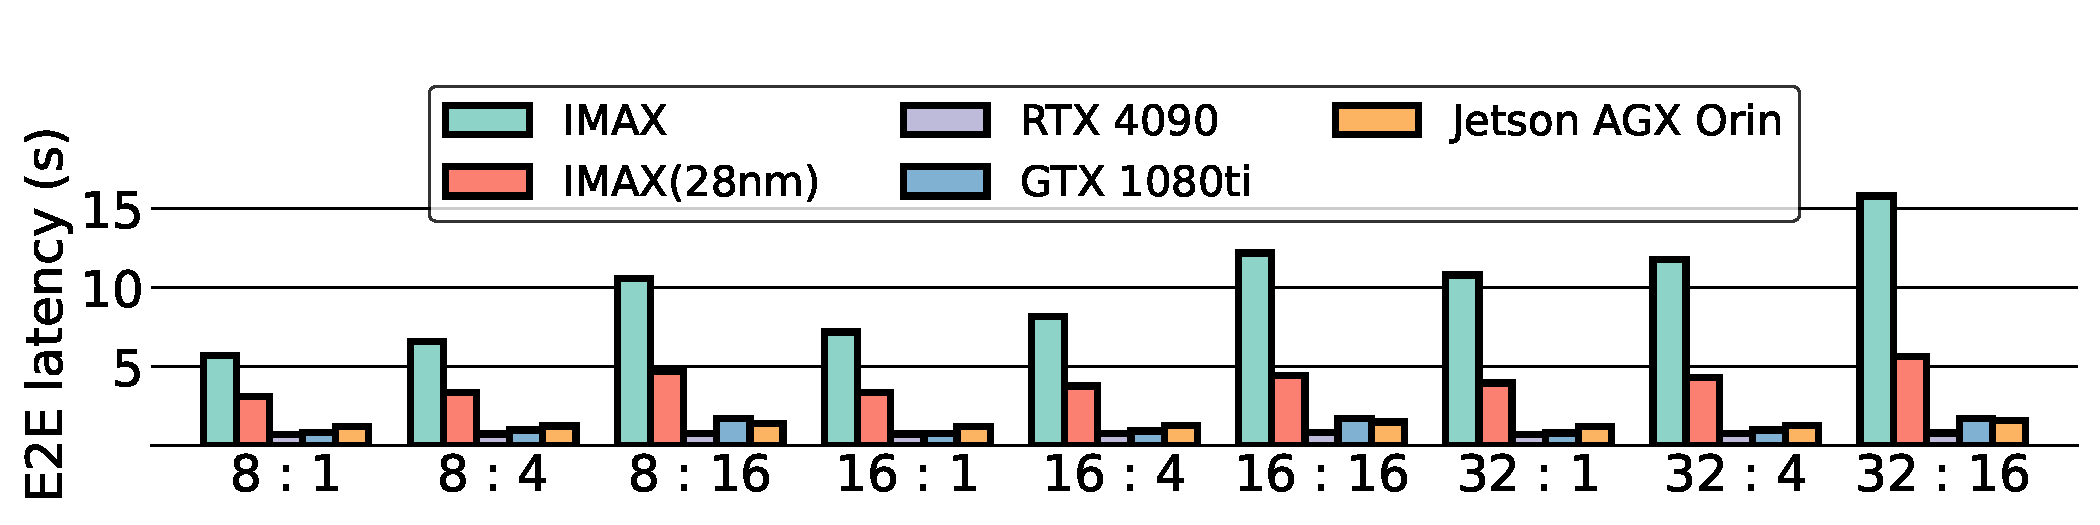
\includegraphics[width=\textwidth]{./E2E_latency_for_Qwen3-0_6B_-_Q3_K_S.pdf}
    \subcaption{Qwen3-0.6B Q3\_K\_S}
    \label{fig:e2e_Qwen3_6B_Q3K_S}
  \end{subfigure}
  
  \vspace{1pt} % 図の間の垂直スペース
  
  % --- (b)の図をsubfigure環境で囲む ---
  \begin{subfigure}{1.0\columnwidth}
    \centering
    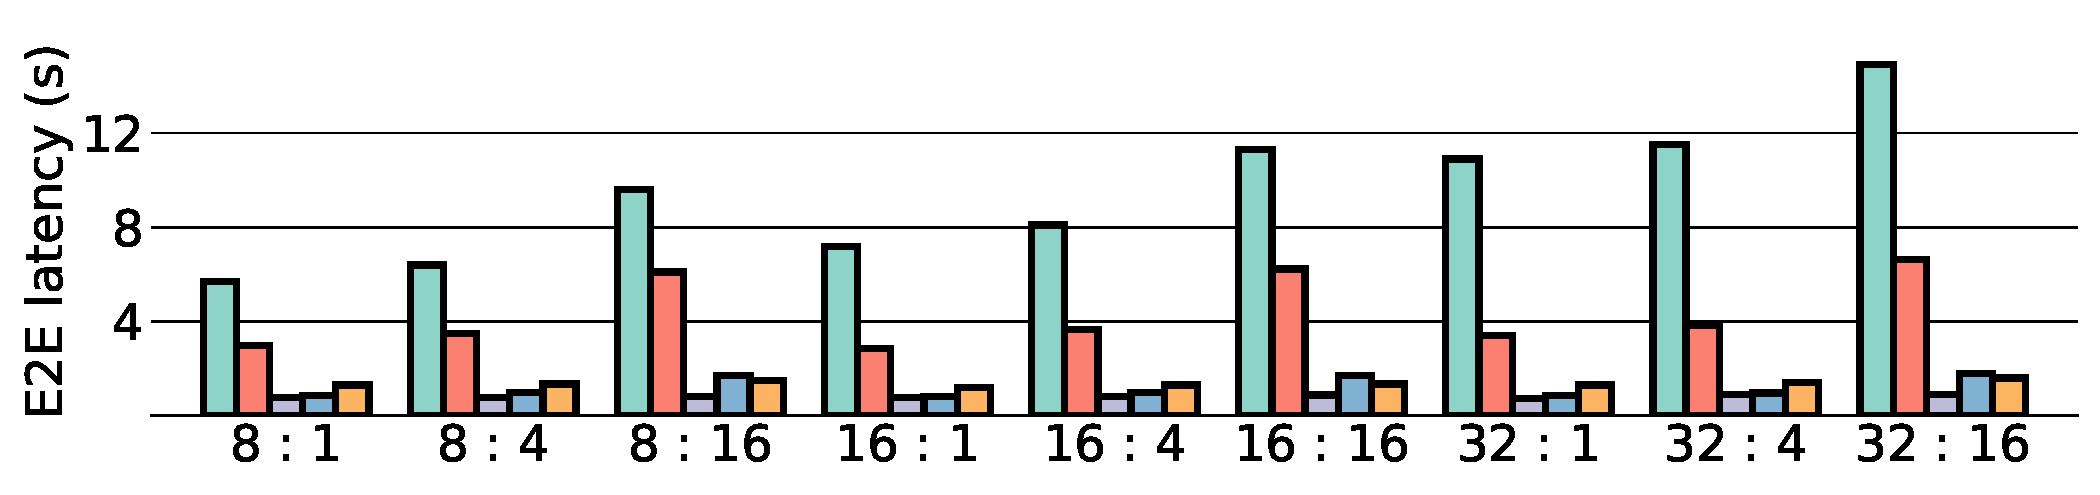
\includegraphics[width=\textwidth]{./E2E_latency_for_Qwen3-0_6B_-_Q8_0.pdf}
    \subcaption{Qwen3-0.6B Q8\_0}
    \label{fig:e2e_Qwen3_6B_Q8_0}
  \end{subfigure}
  
  \vspace{1pt} % 図の間の垂直スペース

    % --- (a)の図をsubfigure環境で囲む ---
    \begin{subfigure}{1.0\columnwidth}
      \centering
      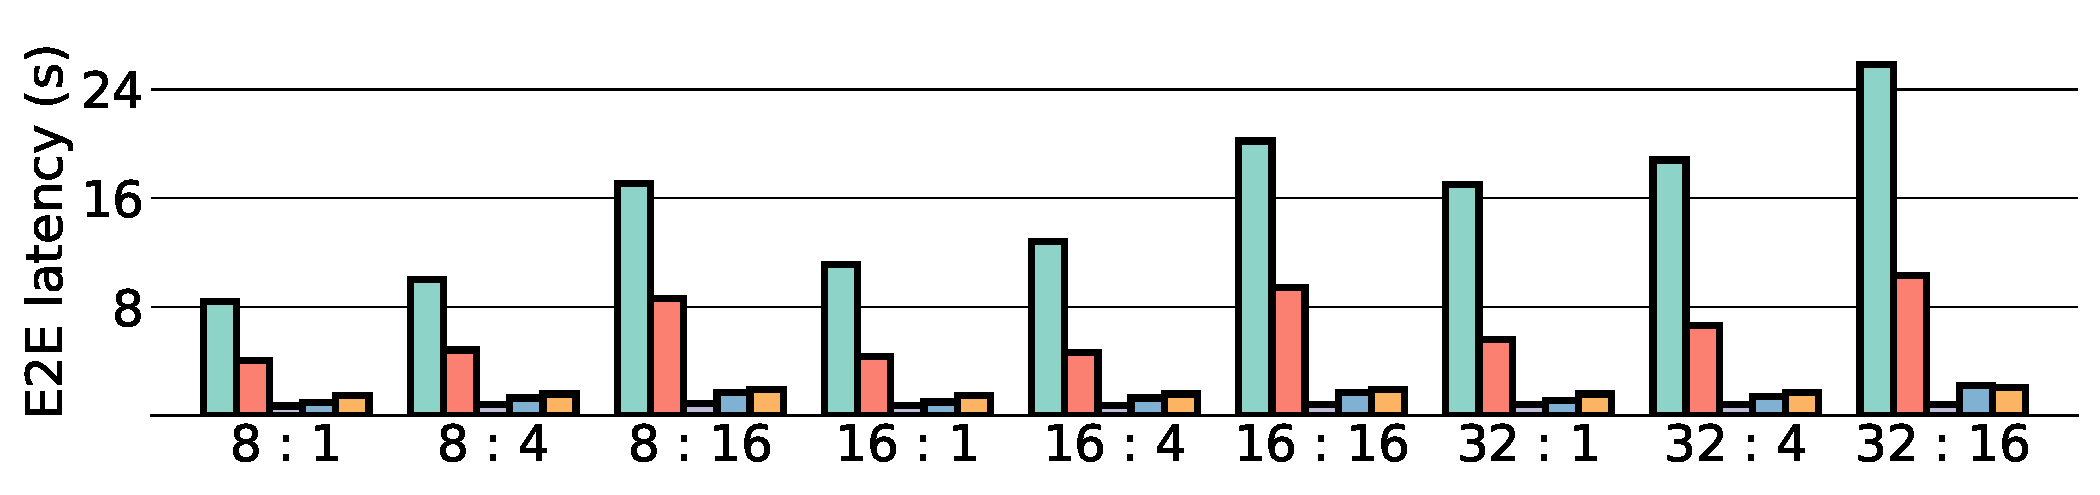
\includegraphics[width=\textwidth]{./E2E_latency_for_Qwen3-1_7B_-_Q3_K_S.pdf}
      \subcaption{Qwen3-1.7B Q3\_K\_S}
      \label{fig:e2e_Qwen3_7B_Q3K_S}
    \end{subfigure}
    
    \vspace{1pt} % 図の間の垂直スペース
    
    % --- (b)の図をsubfigure環境で囲む ---
    \begin{subfigure}{1.0\columnwidth}
      \centering
      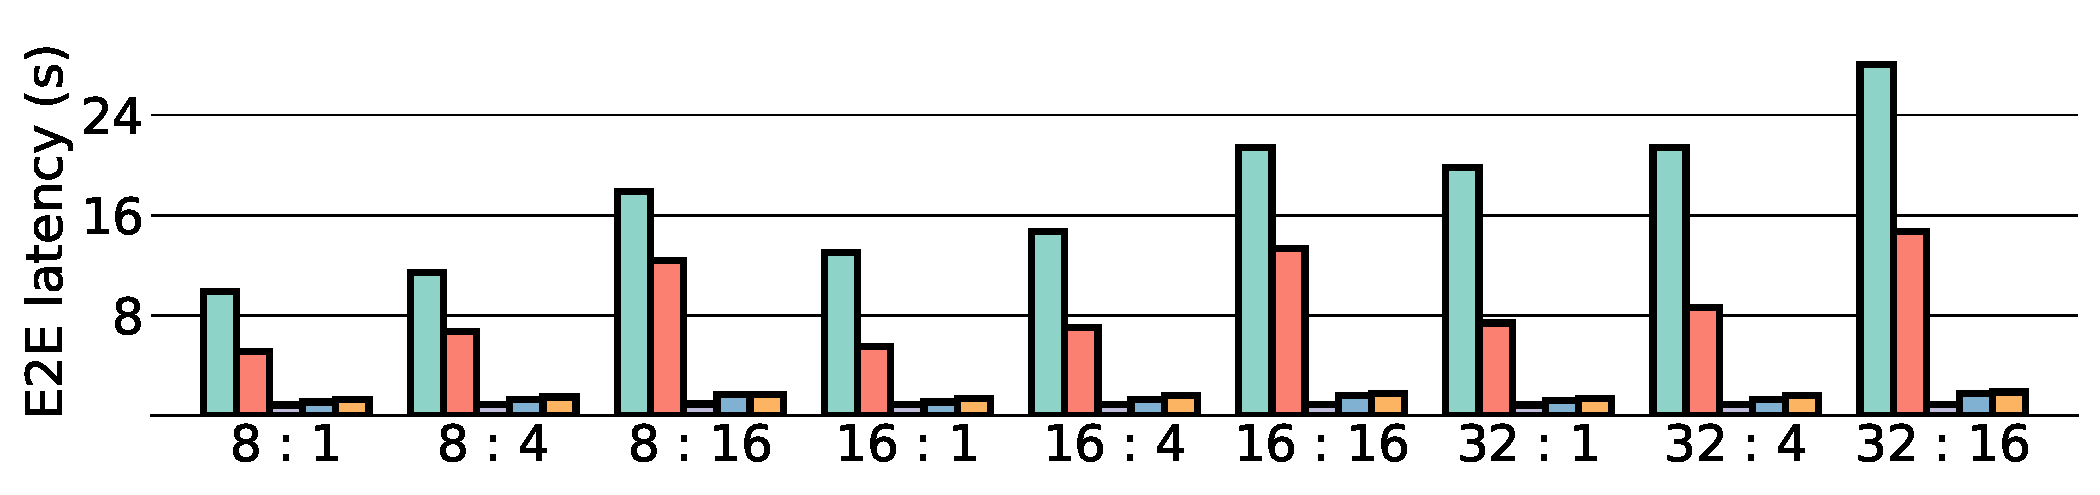
\includegraphics[width=\textwidth]{./E2E_latency_for_Qwen3-1_7B_-_Q8_0.pdf}
      \subcaption{Qwen3-1.7B Q8\_0}
      \label{fig:e2e_Qwen3_7B_Q8_0}
    \end{subfigure}
    
    \vspace{1pt} % 図の間の垂直スペース
  
      % --- (a)の図をsubfigure環境で囲む ---
  \begin{subfigure}{1.0\columnwidth}
    \centering
    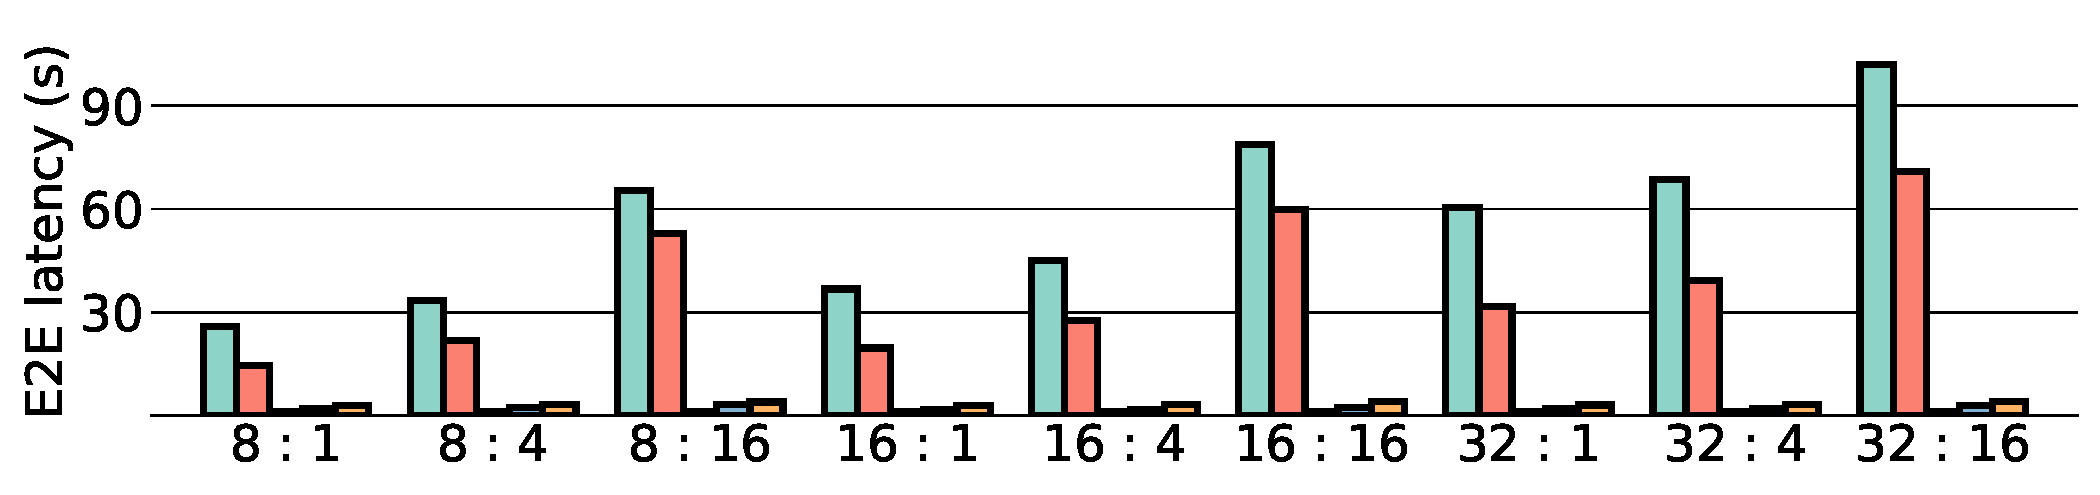
\includegraphics[width=\textwidth]{./E2E_latency_for_Qwen3-8B_-_Q3_K_S.pdf}
    \subcaption{Qwen3-8B Q3\_K\_S}
    \label{fig:e2e_Qwen3_8B_Q3K_S}
  \end{subfigure}
  
  \vspace{1pt} % 図の間の垂直スペース
  
  % --- (b)の図をsubfigure環境で囲む ---
  \begin{subfigure}{1.0\columnwidth}
    \centering
    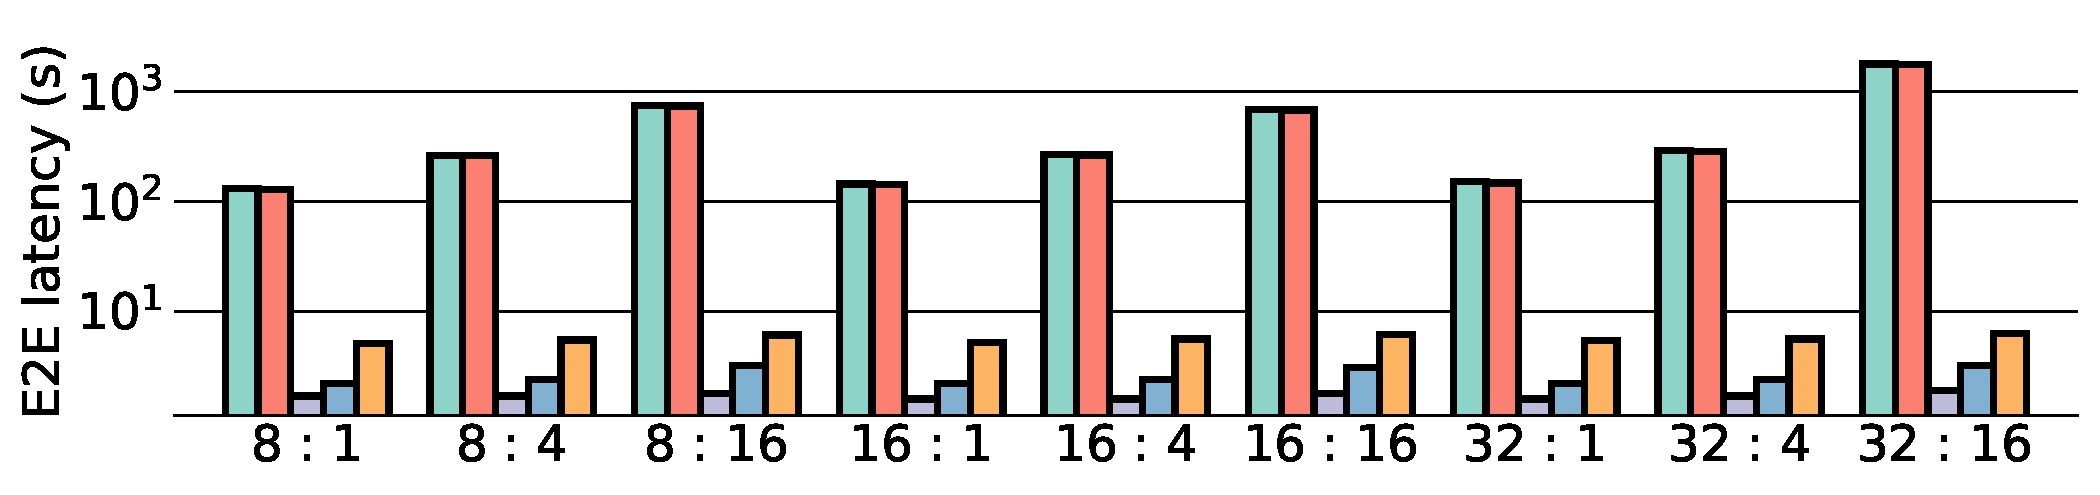
\includegraphics[width=\textwidth]{./E2E_latency_for_Qwen3-8B_-_Q8_0.pdf}
    \subcaption{Qwen3-8B Q8\_0}
    \label{fig:e2e_Qwen3_8B_Q8_0}
  \end{subfigure}
  
  % \vspace{6pt} % 図の間の垂直スペース
  % --- 変更点：メインキャプションを一番下に配置 ---
  \caption{End-to-end performance comparison of E2E latency by device. IMAX is measured in FPGA and IMAX (\SI{28}{\nano\meter}) is projected.}
  \label{fig:e2e_latency}
\end{figure}




\begin{figure}[t]
  \centering

  % --- (b)の図をsubfigure環境で囲む：PDP ---
  \begin{subfigure}{1.0\columnwidth}
    \centering
    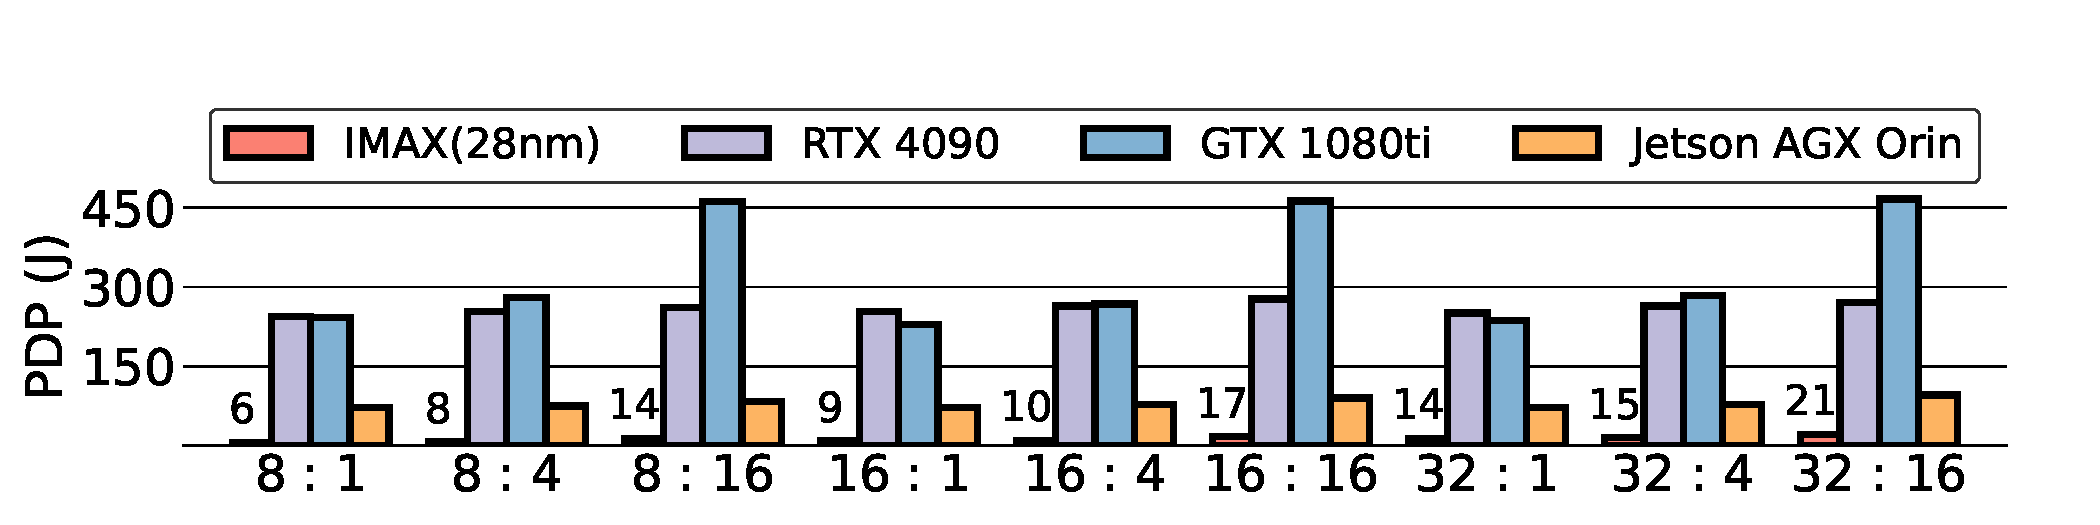
\includegraphics[width=\textwidth]{./PDP_for_Qwen3-0_6B_-_Q3_K_S.pdf}
    \subcaption{Qwen3-0.6B Q3\_K\_S}
    \label{fig:pdp_Qwen3_6B_Q3K_S}
  \end{subfigure}

  \vspace{1pt} % 図の間の垂直スペース

  \begin{subfigure}{1.0\columnwidth}
    \centering
    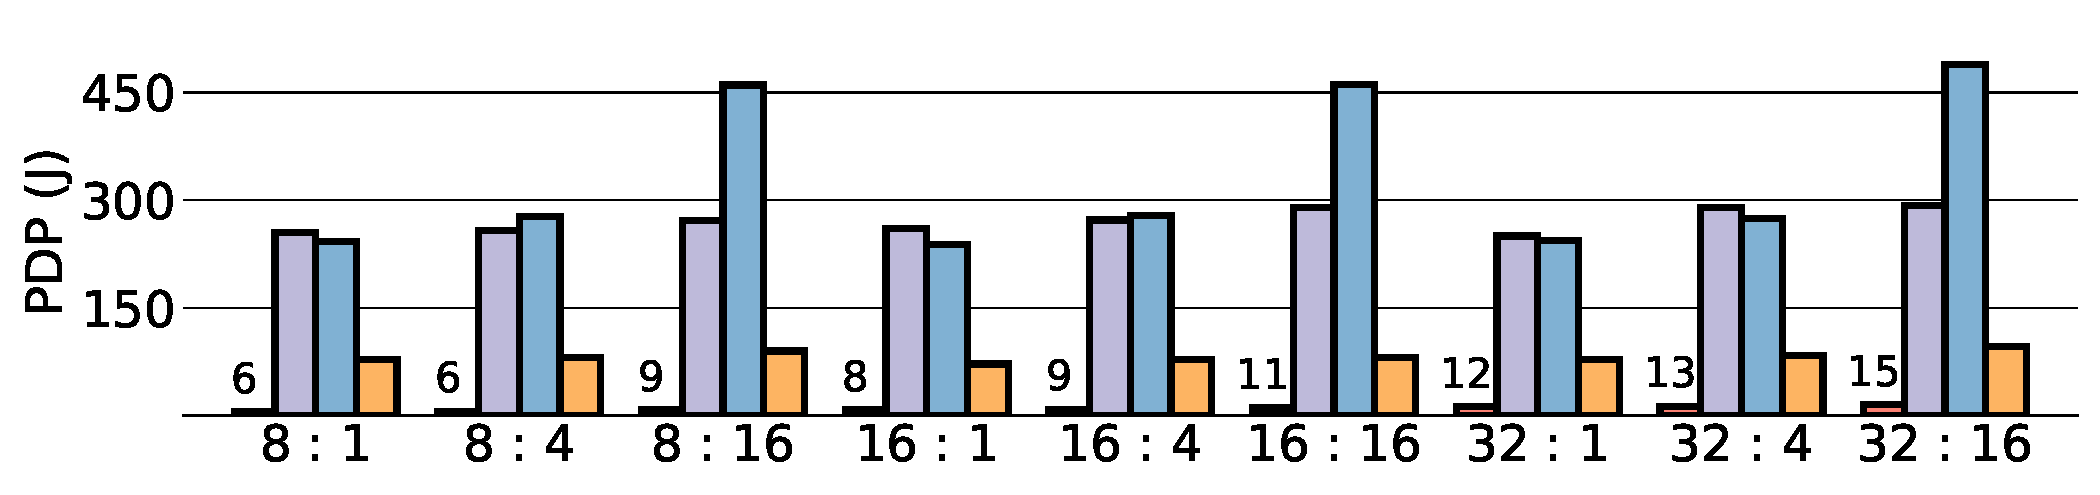
\includegraphics[width=\textwidth]{./PDP_for_Qwen3-0_6B_-_Q8_0.pdf}
    \subcaption{Qwen3-0.6B Q8\_0}
    \label{fig:pdp_Qwen3_6B_Q8_0}
  \end{subfigure}

  % --- (d)の図をsubfigure環境で囲む：PDP ---
  \begin{subfigure}{1.0\columnwidth}
    \centering
    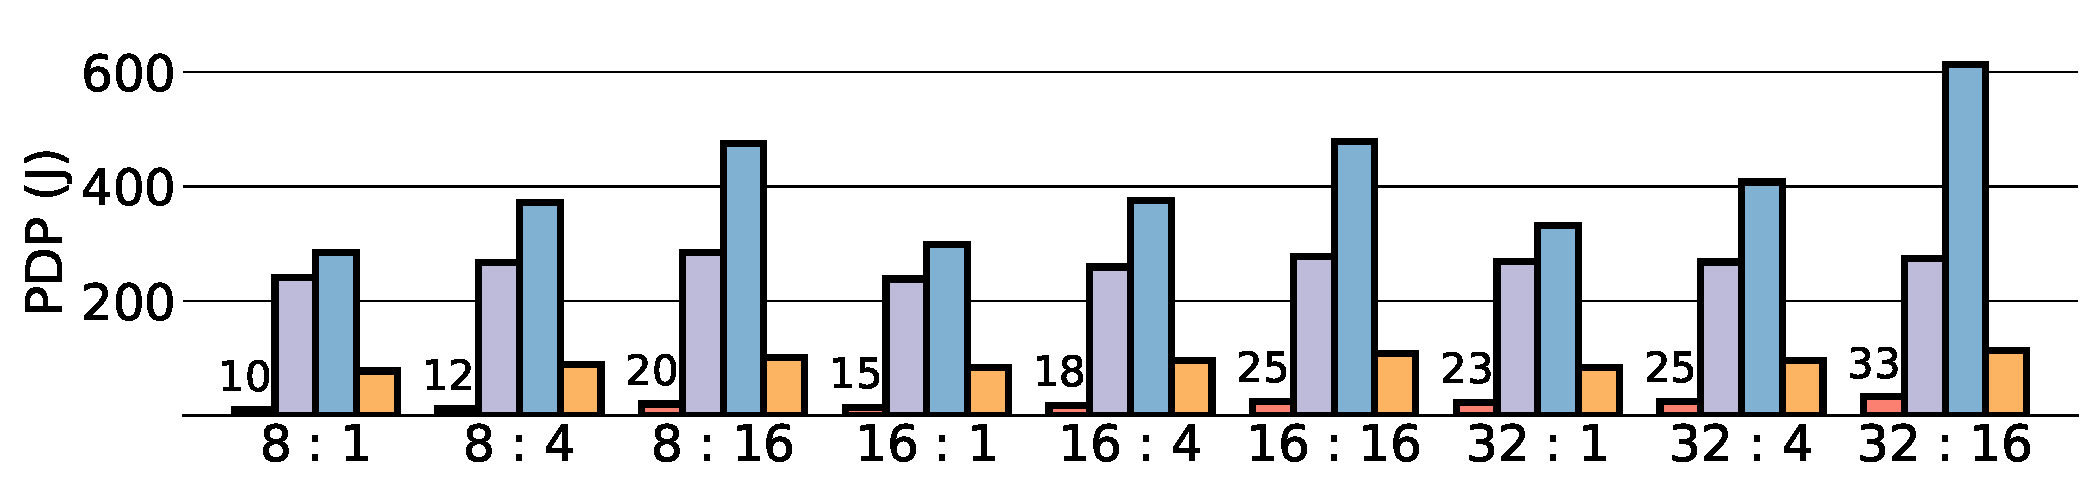
\includegraphics[width=\textwidth]{./PDP_for_Qwen3-1_7B_-_Q3_K_S.pdf}
    \subcaption{Qwen3-1.7B Q3\_K\_S}
    \label{fig:pdp_Qwen3_7B_Q3K_S}
  \end{subfigure}

  \vspace{1pt} % 図の間の垂直スペース

  % --- (e)の図をsubfigure環境で囲む：E2E ---
  \begin{subfigure}{1.0\columnwidth}
    \centering
    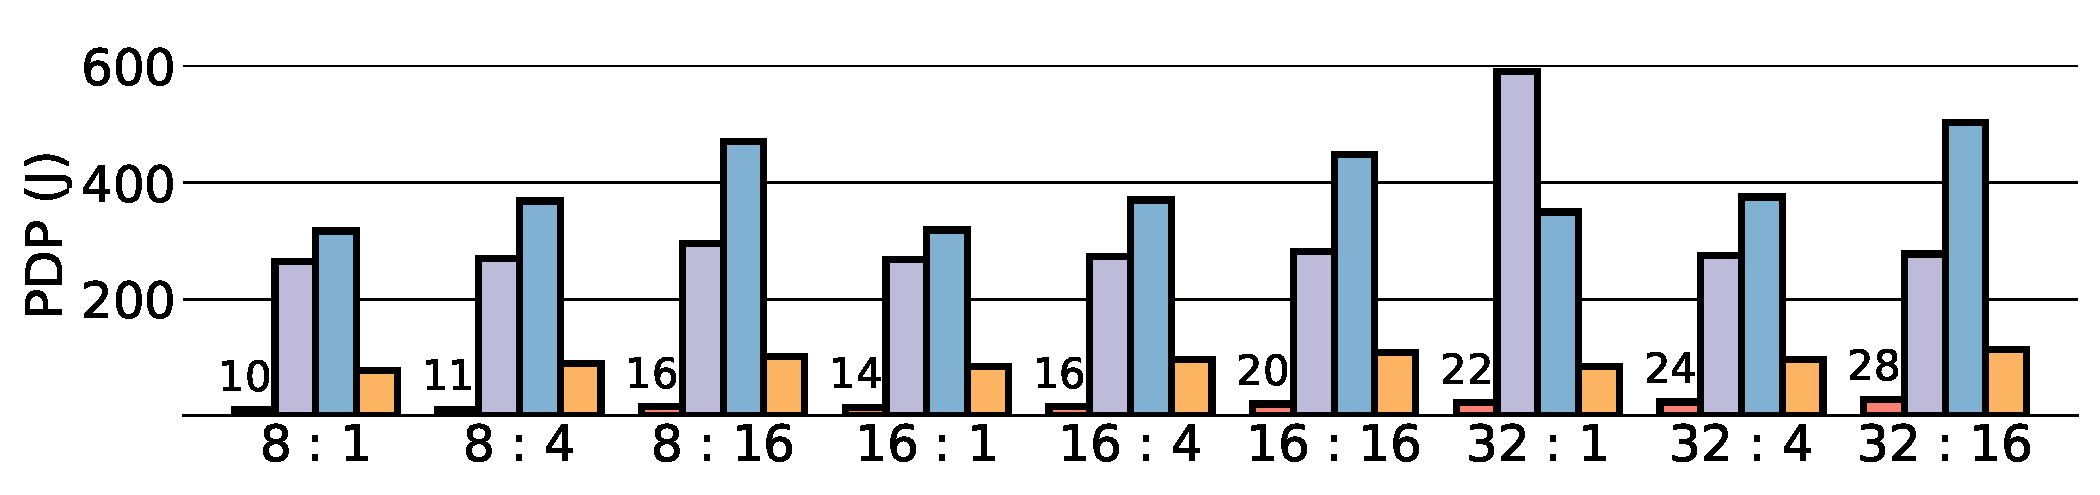
\includegraphics[width=\textwidth]{./PDP_for_Qwen3-1_7B_-_Q8_0.pdf}
    \subcaption{Qwen3-1.7B Q8\_0}
    \label{fig:pdp_Qwen3_7B_Q8_0}
  \end{subfigure}

  \vspace{1pt} % 図の間の垂直スペース

  % --- (f)の図をsubfigure環境で囲む：PDP ---
  \begin{subfigure}{1.0\columnwidth}
    \centering
    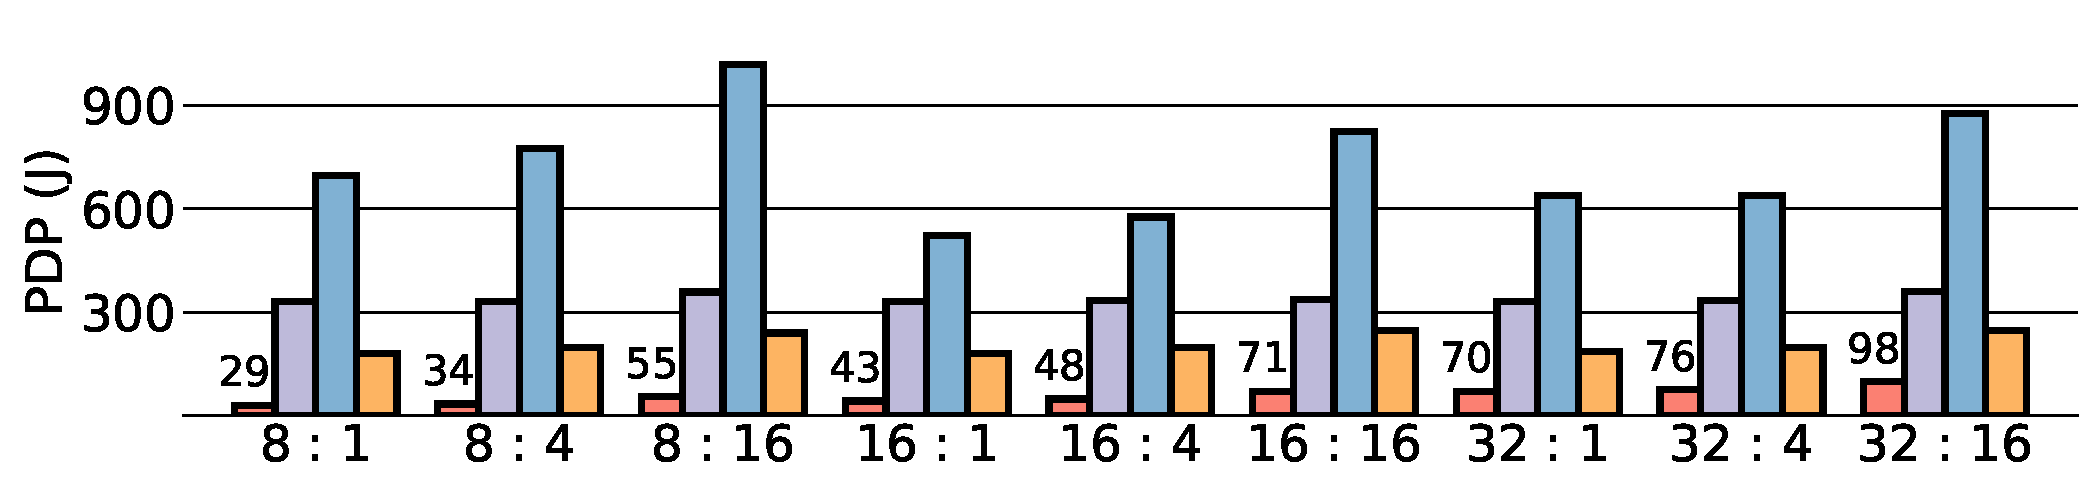
\includegraphics[width=\textwidth]{./PDP_for_Qwen3-8B_-_Q3_K_S.pdf}
    \subcaption{Qwen3-8B Q3\_K\_S}
    \label{fig:pdp_Qwen3_8B_Q3K_S}
  \end{subfigure}

  
  \vspace{1pt} % 図の間の垂直スペース

  % --- (f)の図をsubfigure環境で囲む：PDP ---
  \begin{subfigure}{1.0\columnwidth}
    \centering
    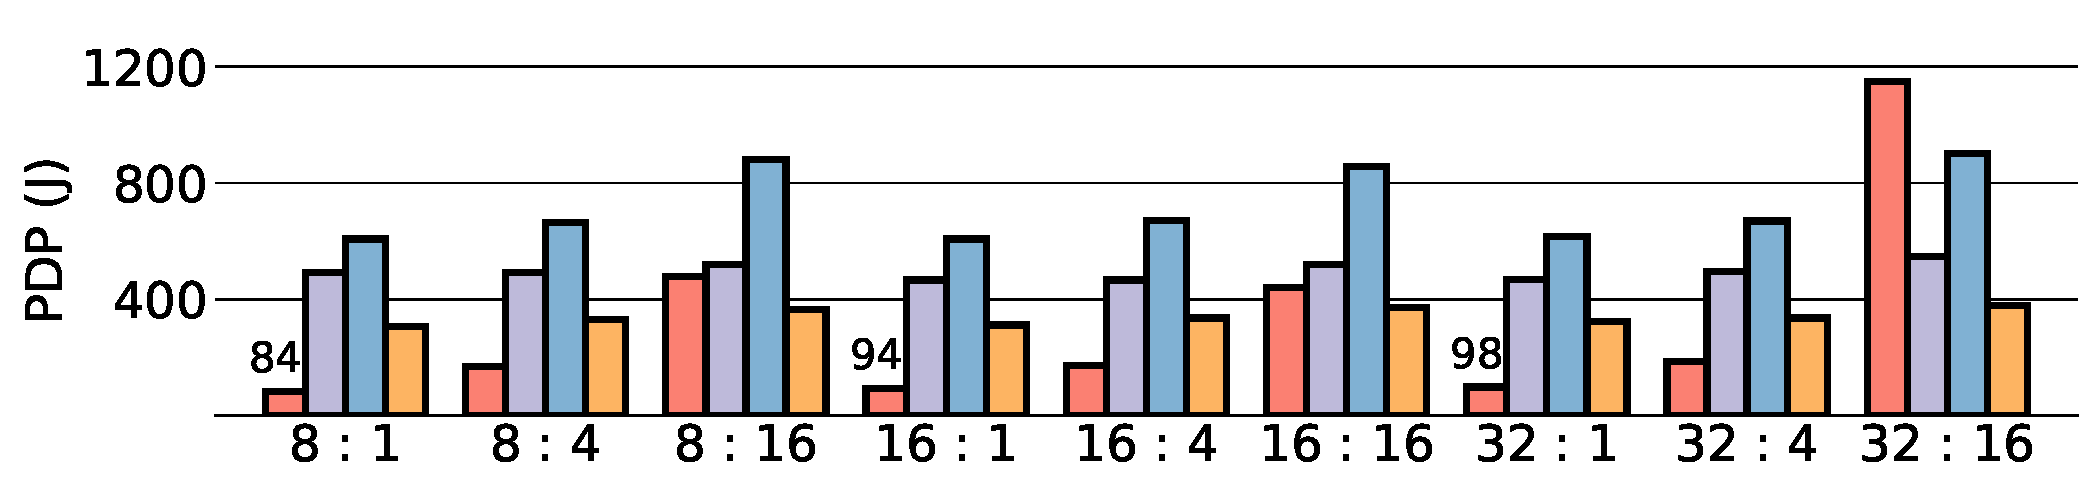
\includegraphics[width=\textwidth]{./PDP_for_Qwen3-8B_-_Q8_0.pdf}
    \subcaption{Qwen3-8B Q8\_0}
    \label{fig:pdp_Qwen3_8B_Q8_0}
  \end{subfigure}
  % \vspace{6pt} % 図の間の垂直スペース
  % --- 変更点：メインキャプションを一番下に配置 ---
  \caption{PDP comparison by device (lower is better). The numeric value for IMAX (\SI{28}{\nano\meter}) is shown when it is below \SI{100} to ensure readability.}
  \label{fig:e2e_pdp_comparison}
\end{figure}

\begin{figure}[t]
  \centering

  % --- (b)の図をsubfigure環境で囲む：PDP ---
  \begin{subfigure}{1.0\columnwidth}
    \centering
    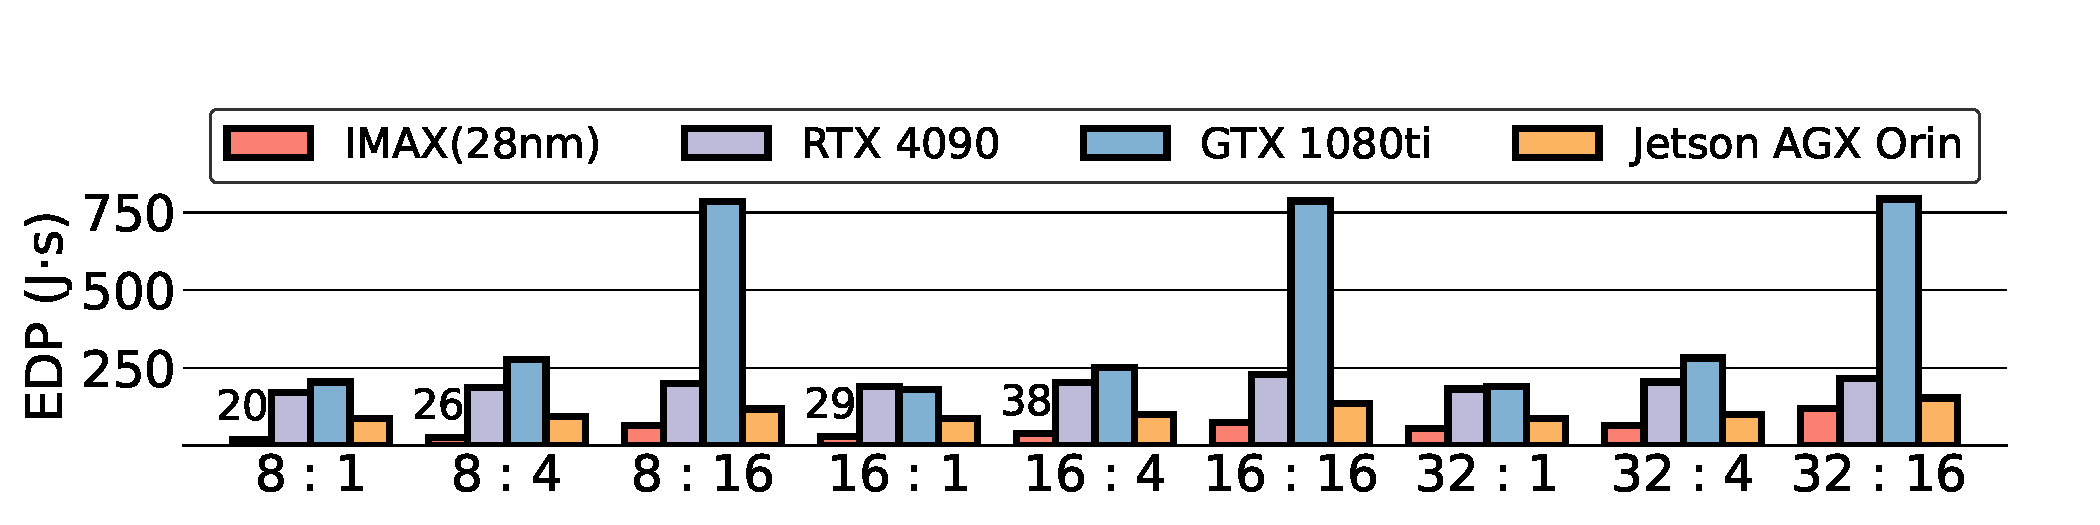
\includegraphics[width=\textwidth]{./EDP_for_Qwen3-0_6B_-_Q3_K_S.pdf}
    \subcaption{Qwen3-0.6B Q3\_K\_S}
    \label{fig:edp_Qwen3_6B_Q3K_S}
  \end{subfigure}

  \vspace{1pt} % 図の間の垂直スペース

  \begin{subfigure}{1.0\columnwidth}
    \centering
    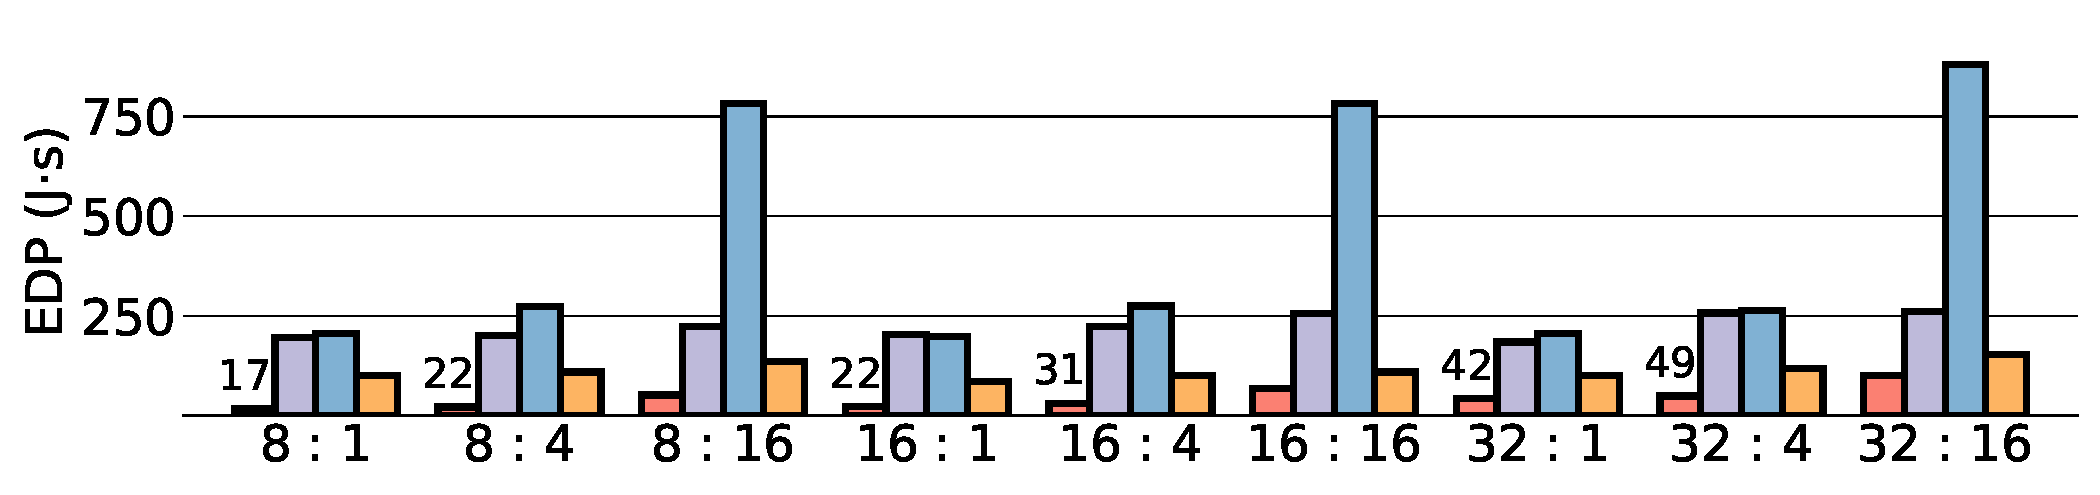
\includegraphics[width=\textwidth]{./EDP_for_Qwen3-0_6B_-_Q8_0.pdf}
    \subcaption{Qwen3-0.6B Q8\_0}
    \label{fig:edp_Qwen3_6B_Q8_0}
  \end{subfigure}

  % --- (d)の図をsubfigure環境で囲む：PDP ---
  \begin{subfigure}{1.0\columnwidth}
    \centering
    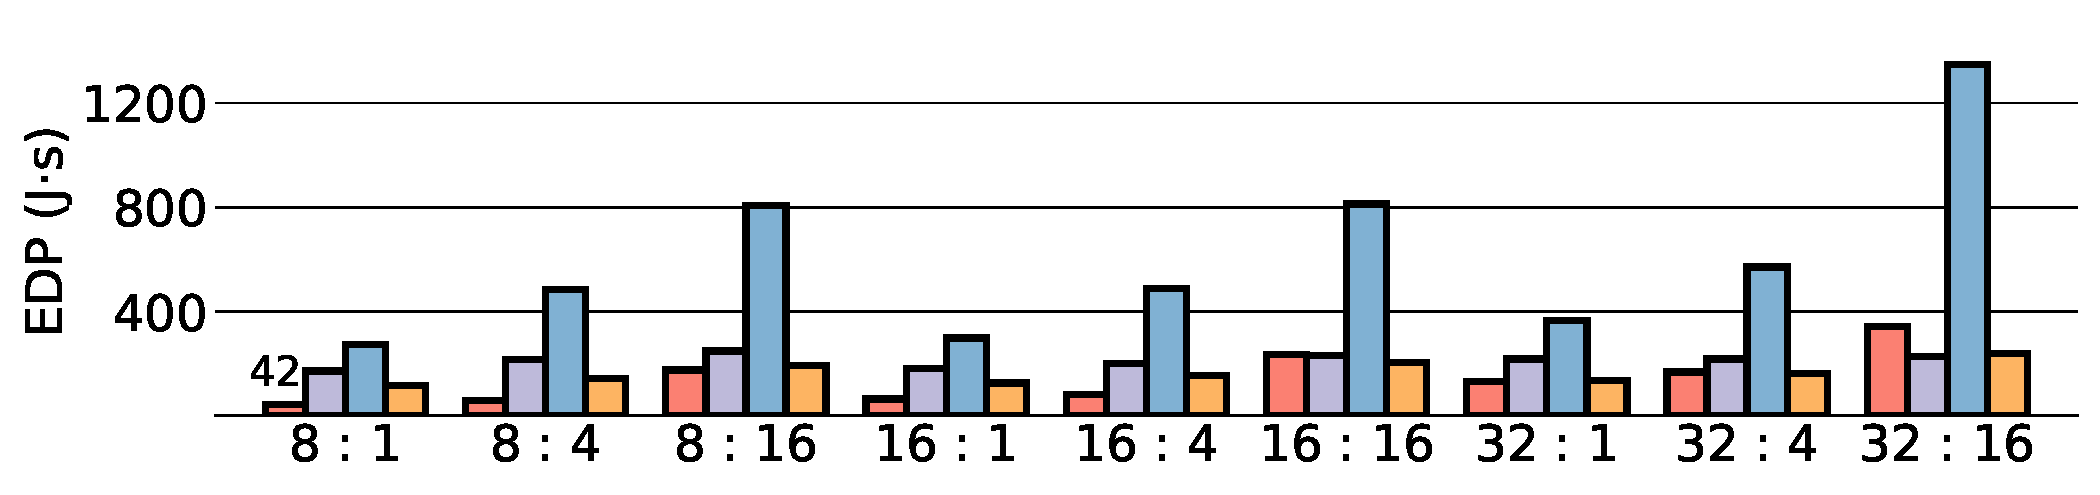
\includegraphics[width=\textwidth]{./EDP_for_Qwen3-1_7B_-_Q3_K_S.pdf}
    \subcaption{Qwen3-1.7B Q3\_K\_S}
    \label{fig:edp_Qwen3_7B_Q3K_S}
  \end{subfigure}

  \vspace{1pt} % 図の間の垂直スペース

  % --- (e)の図をsubfigure環境で囲む：E2E ---
  \begin{subfigure}{1.0\columnwidth}
    \centering
    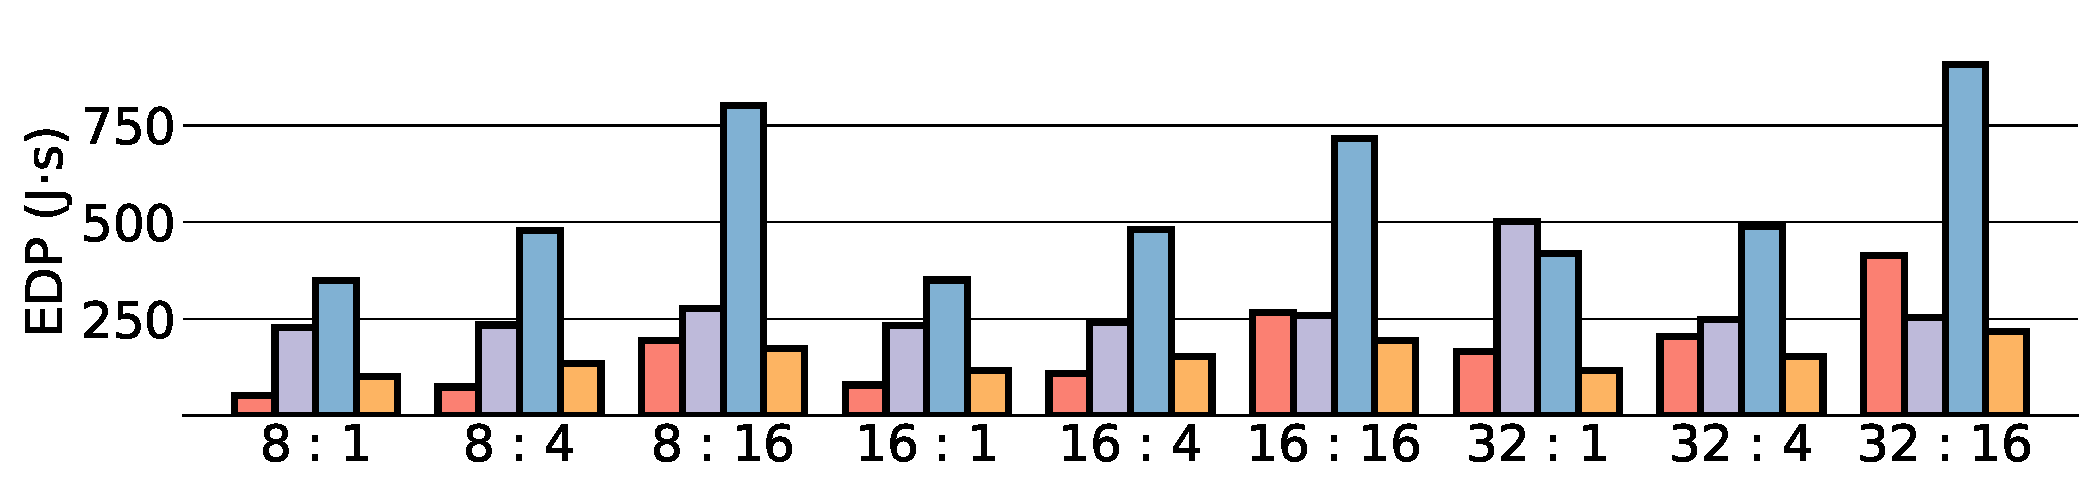
\includegraphics[width=\textwidth]{./EDP_for_Qwen3-1_7B_-_Q8_0.pdf}
    \subcaption{Qwen3-1.7B Q8\_0}
    \label{fig:edp_Qwen3_7B_Q8_0}
  \end{subfigure}

  \vspace{1pt} % 図の間の垂直スペース

  % --- (f)の図をsubfigure環境で囲む：PDP ---
  \begin{subfigure}{1.0\columnwidth}
    \centering
    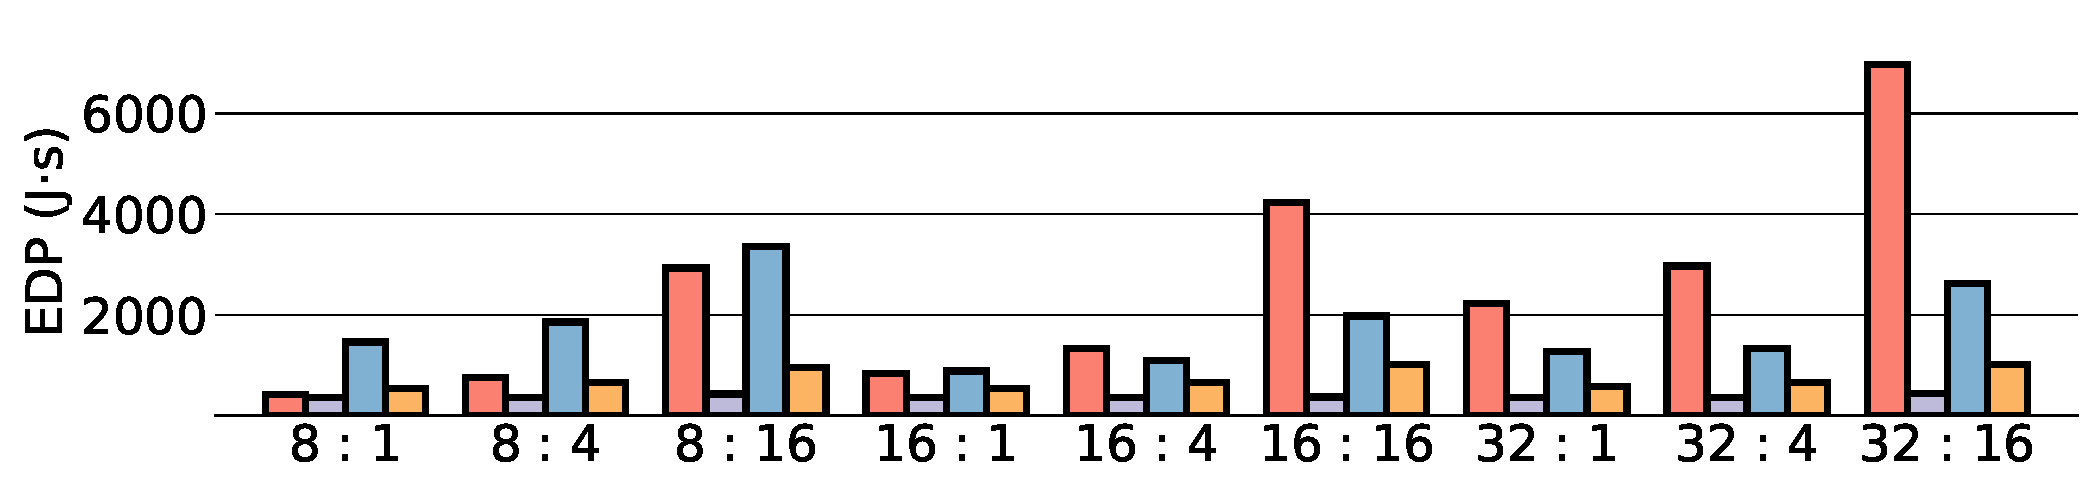
\includegraphics[width=\textwidth]{./EDP_for_Qwen3-8B_-_Q3_K_S.pdf}
    \subcaption{Qwen3-8B Q3\_K\_S}
    \label{fig:edp_Qwen3_8B_Q3K_S}
  \end{subfigure}

  
  \vspace{1pt} % 図の間の垂直スペース

  % --- (f)の図をsubfigure環境で囲む：PDP ---
  \begin{subfigure}{1.0\columnwidth}
    \centering
    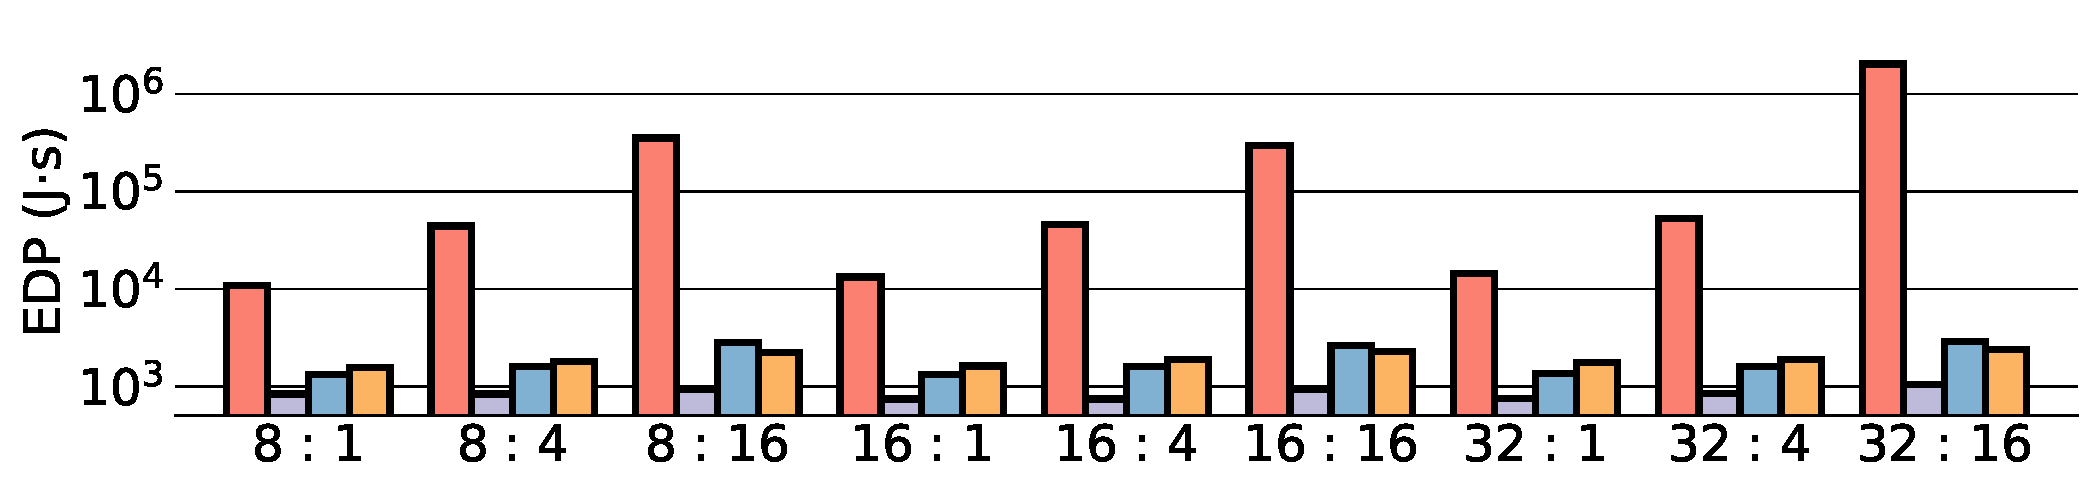
\includegraphics[width=\textwidth]{./EDP_for_Qwen3-8B_-_Q8_0.pdf}
    \subcaption{Qwen3-8B Q8\_0}
    \label{fig:edp_Qwen3_8B_Q8_0}
  \end{subfigure}
  % \vspace{6pt} % 図の間の垂直スペース
  % --- 変更点：メインキャプションを一番下に配置 ---
  \caption{EDP comparison by device (lower is better). The numeric value for IMAX (\SI{28}{\nano\meter}) is shown when it is below \SI{50} to ensure readability.}
  \label{fig:e2e_edp_comparison}
  
\end{figure}


\subsection{E2E Performance Evaluation}
In this subsection, we conduct an E2E performance evaluation of the IMAX architecture. 
We first analyze the E2E latency to assess pure processing speed, then shift our focus to energy efficiency, the primary emphasis of this work, by quantifying the PDP and EDP.


E2E latency comparison in Fig.~\ref{fig:e2e_latency} shows that data transfer has become the primary system bottleneck for our architecture. 
As expected, the NVIDIA RTX 4090 demonstrated the lowest latency in all scenarios due to its substantial resources. 
For instance, on a representative workload, the RTX 4090 achieved a latency of approximately \SI{0.8}{\second}, whereas our projected IMAX (\SI{28}{\nano\meter}) latency was \SI{5.63}{\second}.
Critically, this performance gap scales with model size, particularly for memory-bound models such as Qwen3-8B Q8\_0. 
This scaling behavior strongly indicates that the system's performance is not compute-bound by the IMAX core but is instead bottlenecked by data transfer overhead.


As shown in Fig.~\ref{fig:e2e_pdp_comparison} and Fig.~\ref{fig:e2e_edp_comparison}, the advantages of our design become clear from the energy-centric metrics.
These results indicate that the IMAX architecture, particularly the \SI{28}{\nano\meter} ASIC projection, has the potential to achieve energy efficiency far superior to existing platforms. 
In terms of PDP, the IMAX (\SI{28}{\nano\meter}) projection demonstrates significant advantages. 
For instance, on the compute-bound Qwen3-1.7B Q8\_0 [16:4] workload, IMAX achieved a PDP of just \SI{15.5}{\joule}, outperforming the RTX 4090 (\SI{28.4}{\joule}), GTX 1080 Ti (\SI{35.1}{\joule}), and Jetson (\SI{22.1}{\joule}). 
This represents an efficiency improvement of up to \num{44.4}$\times$, \num{54}$\times$, and \num{13.6}$\times$ over the respective platforms in certain workloads. 
However, this advantage diminishes as data transfer becomes the bottleneck. 
In the most memory-intensive case (Qwen3-8B Q8\_0 [32:16]), the PDP of IMAX surged to \SI{1148.7}{\joule}, which is substantially higher than that of the RTX 4090 (\SI{547.9}{\joule}) and the Jetson (\SI{378.0}{\joule}), highlighting the impact of data transfer overhead on energy consumption.



The EDP evaluation, which squares the impact of execution time, exposes the latency trade-offs of the architecture. 
In compute-bound workloads, the advantage of IMAX (\SI{28}{\nano\meter}) is particularly significant.
For example, on the Qwen3-0.6B Q3\_K\_S [32:16] workload, IMAX (\SI{28}{\nano\meter}) recorded an EDP of \SI{118.9}{\joule\second}, outperforming both the RTX 4090 (\SI{216.8}{\joule\second}) and the Jetson AGX Orin (\SI{153.6}{\joule\second}). 
It maintained a substantial efficiency lead in many scenarios over high-power GPUs, outperforming the RTX 4090 by up to \num{11.5}$\times$ and the GTX 1080 Ti by \num{15}$\times$.
However, as workloads become more memory-bound with larger data transfers, the impact of latency becomes the primary factor.
For the Qwen3-1.7B Q8\_0 [32:16] workload, the shorter latency of the Jetson (\SI{1.9}{\second}) gave it an advantage in EDP, resulting in a score of \SI{216.6}{\joule\second}\, that surpassed IMAX (\SI{413.6}{\joule\second}) with \SI{14.7}{\second}\ latency.
This result indicates the trade-off where low latency is prioritized in EDP, even though IMAX held the advantage in pure energy efficiency (PDP). 
This trend was most significant in the memory-bottlenecked Qwen3-8B Q8\_0 model, where the EDP of IMAX (\SI{28}{\nano\meter}) was substantially higher than that of the other platforms. 
These results suggest that, under the current system configuration, the EDP advantages of the IMAX (\SI{28}{\nano\meter}) architecture are most apparent in compute-bound workloads.

